
\documentclass{beamer}
\usepackage[utf8]{inputenc}

\usetheme{Madrid}
\usecolortheme{default}
\usepackage{amsmath,amssymb,amsfonts,amsthm}
\usepackage{txfonts}
\usepackage{tkz-euclide}
\usepackage{listings}
\usepackage{adjustbox}
\usepackage{array}
\usepackage{tabularx}
\usepackage{gvv}
\usepackage{lmodern}
\usepackage{circuitikz}
\usepackage{tikz}
\usepackage{graphicx}
\usepackage{mathtools}
\setbeamertemplate{page number in head/foot}[totalframenumber]

\usepackage{tcolorbox}
\tcbuselibrary{minted,breakable,xparse,skins}



\definecolor{bg}{gray}{0.95}
\DeclareTCBListing{mintedbox}{O{}m!O{}}{%
  breakable=true,
  listing engine=minted,
  listing only,
  minted language=#2,
  minted style=default,
  minted options={%
    linenos,
    gobble=0,
    breaklines=true,
    breakafter=,,
    fontsize=\small,
    numbersep=8pt,
    #1},
  boxsep=0pt,
  left skip=0pt,
  right skip=0pt,
  left=25pt,
  right=0pt,
  top=3pt,
  bottom=3pt,
  arc=5pt,
  leftrule=0pt,
  rightrule=0pt,
  bottomrule=2pt,
  toprule=2pt,
  colback=bg,
  colframe=orange!70,
  enhanced,
  overlay={%
    \begin{tcbclipinterior}
    \fill[orange!20!white] (frame.south west) rectangle ([xshift=20pt]frame.north west);
    \end{tcbclipinterior}},
  #3,
}
\lstset{
    language=C,
    basicstyle=\ttfamily\small,
    keywordstyle=\color{blue},
    stringstyle=\color{orange},
    commentstyle=\color{green!60!black},
    numbers=left,
    numberstyle=\tiny\color{gray},
    breaklines=true,
    showstringspaces=false,
}


\title 
{1.11.12}
\date{September 9, 2025}


\author 
{Dhanush Kumar A - AI25BTECH11010}



\begin{document}
\frame{\titlepage}
\begin{frame}{Question}
If the sum of two unit vectors is a unit vector, prove that the magnitude of their difference is \(\sqrt{3}\).
\end{frame}
\begin{frame}{Solution}

Let 
	$\vec{u}$ and $\vec{v}$ be unit vectors.\\
	Hence,
\begin{align}
	\vec{u}^T \vec{u} &= 1, & \vec{v}^T \vec{v} &= 1.
\end{align}

\medskip

\begin{align}
||\vec{u}+\vec{v}||^2 &= (\vec{u}+\vec{v})^T(\vec{u}+\vec{v}) \\
&= \vec{u}^T\vec{u} + \vec{v}^T\vec{v} + 2\vec{u}^T\vec{v} \\
1^2 &= 1 + 1 + 2\vec{u}^T\vec{v} \\
1 &= 2 + 2\vec{u}^T\vec{v} \\
\Rightarrow \quad \vec{u}^T\vec{v} &= -\tfrac{1}{2}.
\end{align}

\medskip
\end{frame}
\begin{frame}{Solution}


Now,  
\begin{align}
||\vec{u}-\vec{v}||^2 &= (\vec{u}-\vec{v})^T(\vec{u}-\vec{v}) \\
&= \vec{u}^T\vec{u} + \vec{v}^T\vec{v} - 2\vec{u}^T\vec{v} \\
&= 1 + 1 - 2\left(-\tfrac{1}{2}\right) \\
&= 2 + 1 = 3.
\end{align}

Therefore,  
\begin{align}
||\vec{u}-\vec{v}|| = \sqrt{3}.
\end{align}
\end{frame}
\begin{frame}[fragile]                            
\frametitle{Python code - Verfiying }                
\begin{lstlisting}
import numpy as np
import matplotlib.pyplot as plt

def check_unit_sum_and_plot(a, b):
    # Ensure vectors are unit vectors
    a = a / np.linalg.norm(a)
    b = b / np.linalg.norm(b)
    
    # Compute vectors
    sum_vec = a + b
    diff_vec = a - b
    neg_b = -b
    
    # Magnitudes
    sum_mag = np.linalg.norm(sum_vec)
    diff_mag = np.linalg.norm(diff_vec)
    neg_b_mag = np.linalg.norm(neg_b)  # should be 1 since b is unit
\end{lstlisting}

    \end{frame}
\begin{frame}[fragile]                            
\frametitle{Python code - Verfiying}                
\begin{lstlisting}
 
    print(f"|a+b| = {sum_mag:.3f}")
    print(f"|a-b| = {diff_mag:.3f}")
    print(f"|−b|  = {neg_b_mag:.3f}")

   

\end{lstlisting}
\end{frame}

\begin{frame}[fragile]                            
\frametitle{Python code - Plotting the Vectors}                
\begin{lstlisting}
# Plot
    fig, ax = plt.subplots(figsize=(6,6))
    
    # Function to plot vectors
    def plot_vec(v, color, label):
        ax.arrow(0, 0, v[0], v[1], head_width=0.1, head_length=0.1,
                 fc=color, ec=color, length_includes_head=True)
        ax.text(v[0]*1.1, v[1]*1.1, f"{label}\n|{label}|={np.linalg.norm(v):.2f}", 
                color=color, fontsize=10, ha="center")
    
    # Plot all vectors
    plot_vec(a, "blue", "a")
    plot_vec(b, "green", "b")
    plot_vec(neg_b, "orange", "-b")
    plot_vec(sum_vec, "red", "a+b")
    plot_vec(diff_vec, "purple", "a-b")
   \end{lstlisting}
\end{frame}

\begin{frame}[fragile]                            
\frametitle{Python code - Plotting the Vectors}                
\begin{lstlisting}
 
    # Plot X and Y axes
    ax.axhline(0, color="black", linewidth=1)  # X-axis
    ax.axvline(0, color="black", linewidth=1)  # Y-axis
    
    ax.set_xlim(-2, 2)
    ax.set_ylim(-2, 2)
    ax.set_aspect("equal")
    ax.grid(True, linestyle="--", alpha=0.6)
    ax.set_title("Vectors a, b, -b, a+b, a-b with magnitudes and axes")
    
    # Save figure
    plt.savefig('../figs/vectors_plot.png', dpi=300, bbox_inches="tight")
    plt.show()

# Example: pick a along x-axis, b rotated by 120°
theta = 120 * np.pi / 180
a = np.array([1, 0])
b = np.array([np.cos(theta), np.sin(theta)])

check_unit_sum_and_plot(a, b)
\end{lstlisting}


\end{frame}
\begin{frame}{Plot-Using  Python}
    \centering
    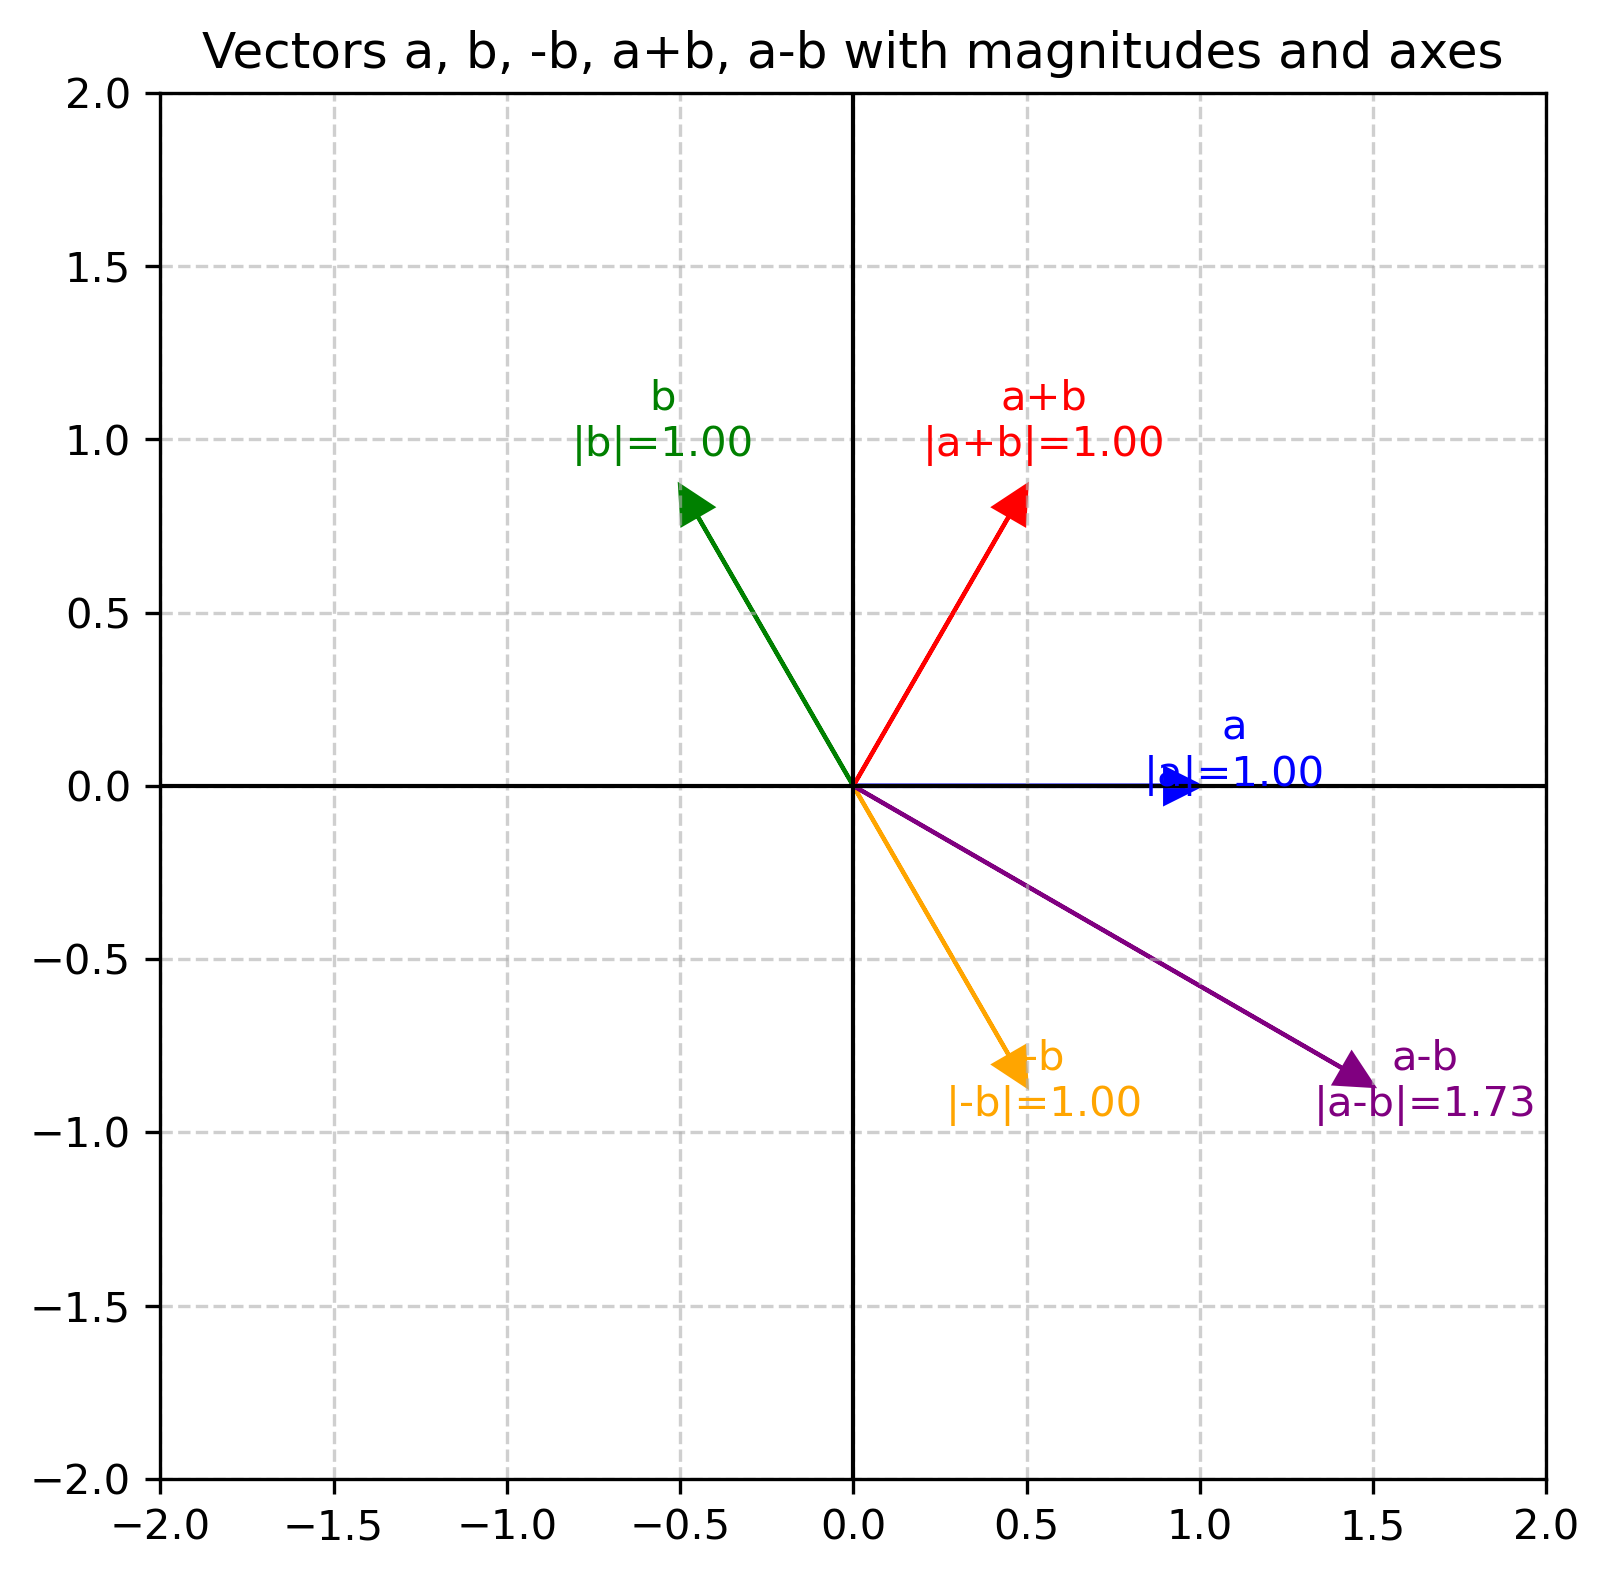
\includegraphics[width=\columnwidth, height=0.8\textheight, keepaspectratio]{../figs/vectors_plot.png}     
\end{frame}


\begin{frame}[fragile]                            
\frametitle{C code - To Verify and Save vectors}                
\begin{lstlisting}
#include <stdio.h>
#include <stdlib.h>
#include <math.h>
#include "/home/dhanush-kumar-a/ee1030-2025/ai25btech11010/matgeo/1.11.12/codes/libs/matfun.h"

int main() {
    // Vectors as 2x1 matrices
    double **a = createMat(2,1);
    double **b = createMat(2,1);

    a[0][0] = 1.0;  a[1][0] = 0.0;  
    b[0][0] = cos(M_PI * 120.0 / 180.0);  
    b[1][0] = sin(M_PI * 120.0 / 180.0);

    // Normalize
    a = Matunit(a, 2);
    b = Matunit(b, 2);
\end{lstlisting}


\end{frame}


\begin{frame}[fragile]                            
\frametitle{C code - To Verify and Save vectors}                
\begin{lstlisting}

    // Operations
    double **sum = Matadd(a, b, 2, 1);
    double **diff = Matsub(a, b, 2, 1);
    double **neg_b = Matscale(b, 2, 1, -1);

    // Magnitudes
    printf("|a+b| = %.3f\n", Matnorm(sum, 2));
    printf("|a-b| = %.3f\n", Matnorm(diff, 2));
    printf("|-b|  = %.3f\n", Matnorm(neg_b, 2));

    // Save results to file
    FILE *fp = fopen("vectors_data.dat", "w");
    if (fp == NULL) {
        printf("Error opening file!\n");
        return 1;
\end{lstlisting}


\end{frame}


\begin{frame}[fragile]                            
\frametitle{C code - To Verify and Save vectors}                
\begin{lstlisting}


    }
    fprintf(fp, "Vector\tX\tY\tMagnitude\n");
    fprintf(fp, "a\t%.4f\t%.4f\t%.4f\n", a[0][0], a[1][0], Matnorm(a,2));
    fprintf(fp, "b\t%.4f\t%.4f\t%.4f\n", b[0][0], b[1][0], Matnorm(b,2));
    fprintf(fp, "-b\t%.4f\t%.4f\t%.4f\n", neg_b[0][0], neg_b[1][0], Matnorm(neg_b,2));
    fprintf(fp, "a+b\t%.4f\t%.4f\t%.4f\n", sum[0][0], sum[1][0], Matnorm(sum,2));
    fprintf(fp, "a-b\t%.4f\t%.4f\t%.4f\n", diff[0][0], diff[1][0], Matnorm(diff,2));
    fclose(fp);

    printf("Data saved to vectors_data.dat\n");
    return 0;
}

\end{lstlisting}
\end{frame}

	
\begin{frame}[fragile]                              
	\frametitle{Python code -Ploting the Vector using c function} 
	\begin{lstlisting}
import os
import numpy as np
import matplotlib.pyplot as plt

# Step 1: Compile the C program
os.system("gcc c.c -o vectors -lm")

# Step 2: Run the compiled C program
os.system("./vectors")

# Step 3: Load data (skip header row, read mixed types)
data = np.genfromtxt("vectors_data.dat", skip_header=1, dtype=None, encoding="utf-8")

# Separate columns
labels = [row[0] for row in data]   # first column is text
x_vals = np.array([float(row[1]) for row in data])
y_vals = np.array([float(row[2]) for row in data])
mags   = np.array([float(row[3]) for row in data])
\end{lstlisting}
\end{frame}

	
\begin{frame}[fragile]                              
	\frametitle{Python code -Ploting the Vector using c function} 
	\begin{lstlisting}

# Step 4: Plot vectors
fig, ax = plt.subplots(figsize=(6,6))

for label, x, y, mag in zip(labels, x_vals, y_vals, mags):
    ax.arrow(0, 0, x, y, head_width=0.1, head_length=0.1,
             fc="blue", ec="blue", alpha=0.7, length_includes_head=True)
    ax.text(x*1.1, y*1.1, f"{label}\n|{label}|={mag:.2f}", fontsize=10, ha="center")

# Plot x and y axes
ax.axhline(0, color="black", linewidth=1.0, linestyle="--")  # X-axis
ax.axvline(0, color="black", linewidth=1.0, linestyle="--")  # Y-axis
\end{lstlisting}
\end{frame}

	
\begin{frame}[fragile]                              
	\frametitle{Python code -Ploting the Vector using c function} 
	\begin{lstlisting}

# Formatting
ax.set_xlim(-2, 2)
ax.set_ylim(-2, 2)
ax.set_aspect("equal")
ax.grid(True)
ax.set_title("Vectors from C Program with X and Y Axes")

# Save and show plot
plt.savefig("../figs/vectors_from_c.png", dpi=300, bbox_inches="tight")
plt.show()


\end{lstlisting}                               
\end{frame}

\begin{frame}{Plot-Using  Python and C}
    \centering
    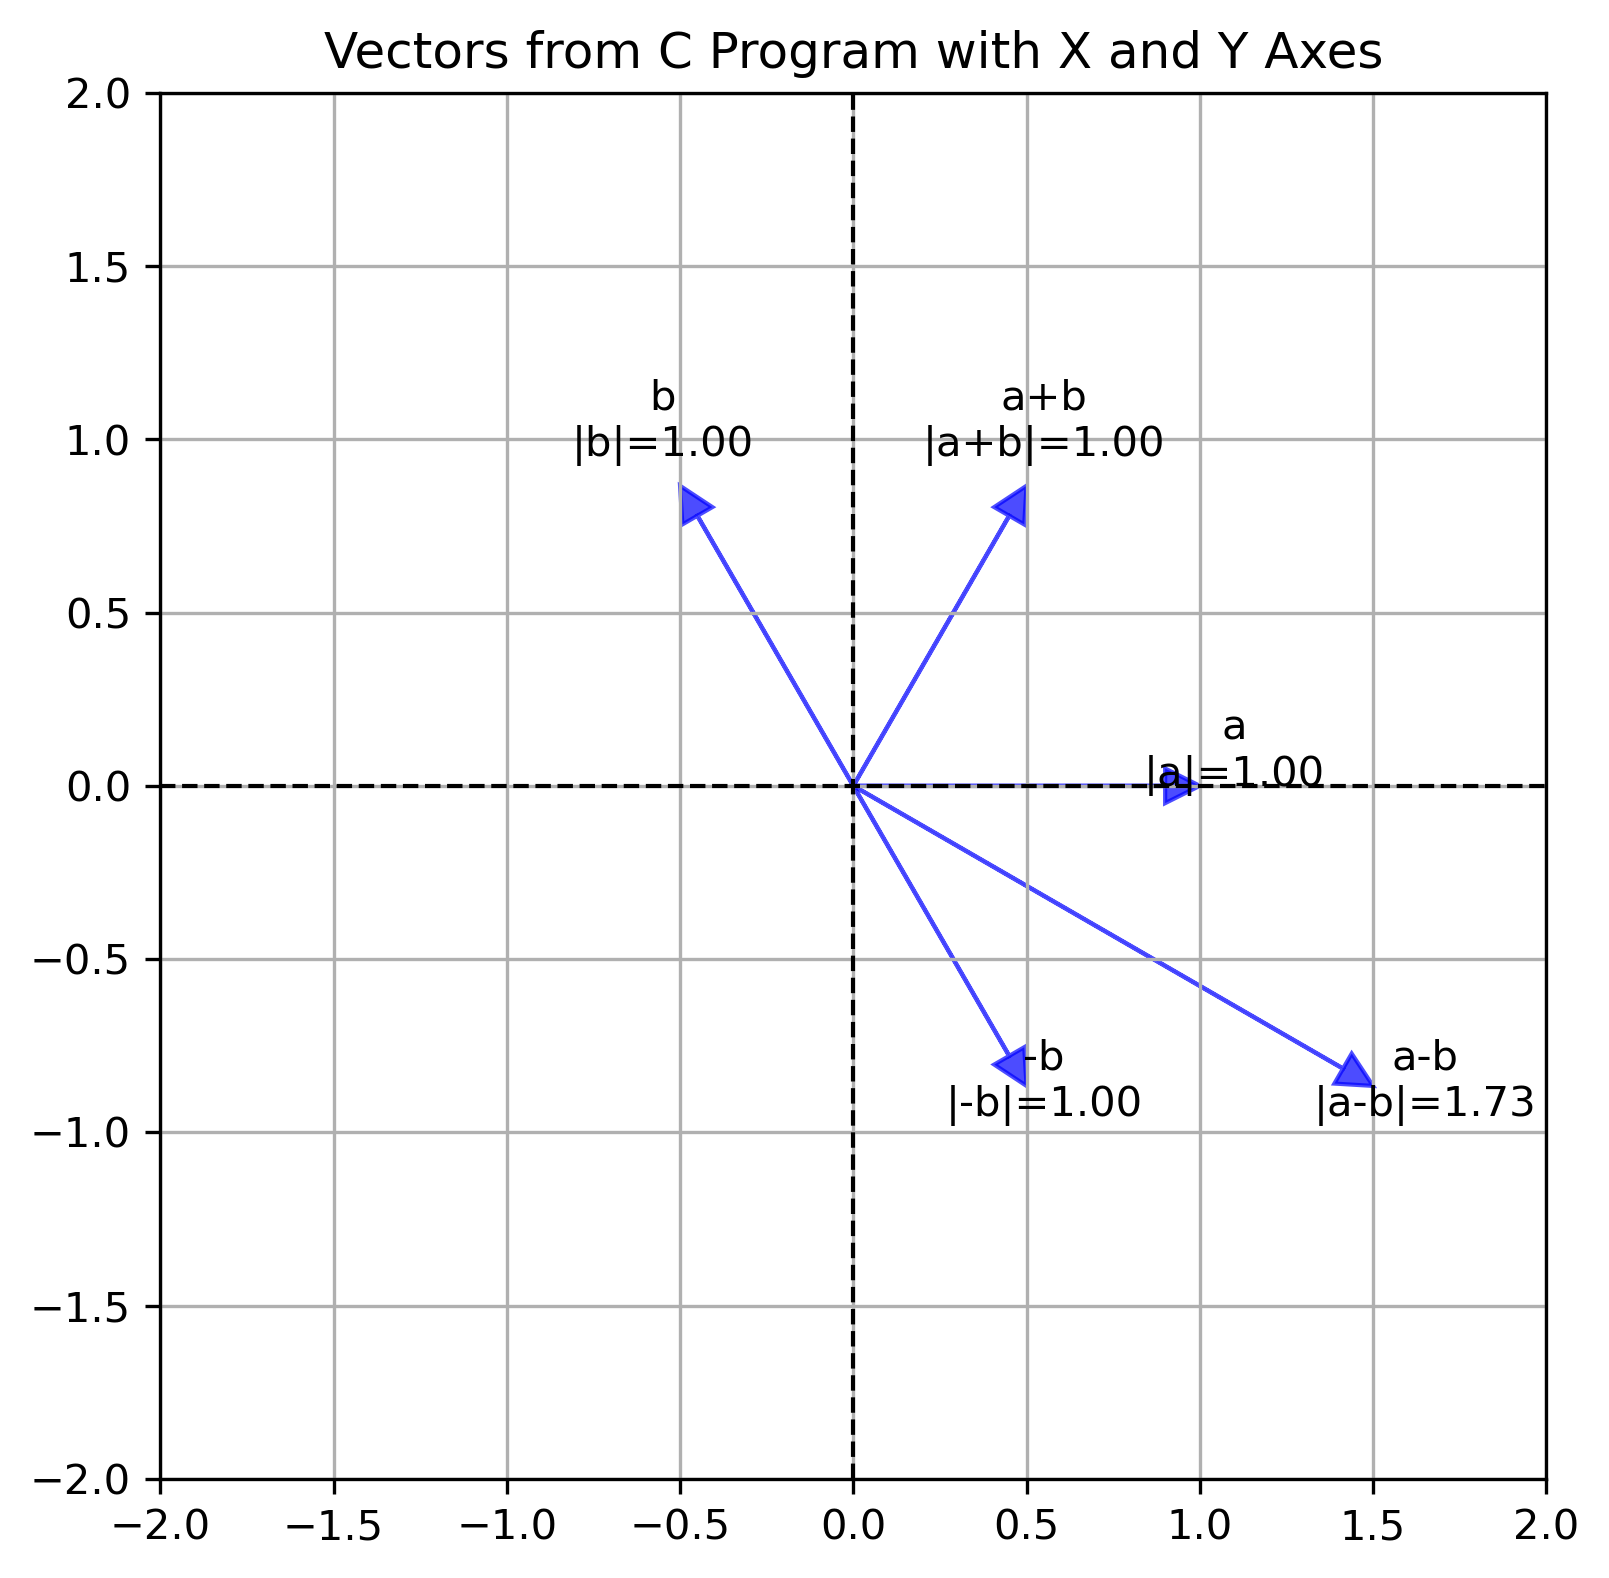
\includegraphics[width=\columnwidth, height=0.8\textheight, keepaspectratio]{../figs/vectors_from_c.png}     
\end{frame}

	


\end{document}

